
\paragraph{Annotation}
Responses were left unannotated for the number of verbs when it was impossible to determine the number of verb phrases, primarily due to ungrammaticality beyond unambigously recoverable orthographic issues.
In the English study, a fraction of subjects produced some or mostly ungrammatical completions; 17.6\% of responses remained unannotated due to such issues.
Such issues were not prominent in the other languages; 0\% of Spanish and 2.3\% of German responses remained unannotated.

\paragraph{Analysis and Results}


Logistic mixed-effects models were similar to those used for reading times (Section~\ref{sec:regression-details}):
Covariance matrices for random effects were parameterized as the combination of a correlation matrix and a vector of standard deviations \citep{barnard2000modeling}.
We used a flat prior for the fixed effect coefficient, a Student's $t$ prior with 3 degrees of freedom, location 0, and scale 2.5 for the intercept and the standard deviations, and an LKJ(1) prior for the random effects correlation matrices.
We show posteriors of the analyses reported in the main paper in Figure~\ref{fig:production-posteriors}.

See further Figure~\ref{fig:production-posteriors-corpora} for English results when estimating Embedding Bias on two other large corpora of English.


\begin{figure}	
	\begin{tabular}{ccc}
		English (Wikipedia) & German & Spanish \\
		\includegraphics[width=0.3\textwidth]{../resource-rational-surprisal/experiments/production/experiment3_english/Submiterator-master/figures/posterior-histograms.pdf} 
		&
		\includegraphics[width=0.3\textwidth]{../resource-rational-surprisal/experiments/production/experiment3_german/Submiterator-master/figures/posterior-histograms.pdf} 
		&
		\includegraphics[width=0.3\textwidth]{../resource-rational-surprisal/experiments/production/experiment3_spanish/Submiterator-master/figures/posterior-histograms.pdf} 
	\end{tabular}

	\caption{Posteriors for trial-by-trial logistic mixed-effects analyses of the production studies. The dependent variable is whether less than three verbs were produced. Variation in the intercepts reflects differences in the overall rate of incorrect responses; in particular, it is reduced in German in line with prior findings on center embeddings. The effect of interest is the effect of Embedding Bias, which is estimated at similar magnitude in all languages.}\label{fig:production-posteriors}
\end{figure}



